\documentclass{beamer}

\mode<presentation>
{
  \setbeamertemplate{navigation symbols}{}
  \setbeamertemplate{caption}[numbered]
  \setbeamertemplate{footline}[frame number]
} 
% \beamertemplatenavigationsymbolsempty

\usepackage[english]{babel}
\usepackage[utf8]{inputenc}
\usepackage{natbib}

% \usepackage{lipsum}

\usepackage{mathtext}
\usepackage[T2A]{fontenc}

\setcounter{tocdepth}{1}

\usepackage{amsmath,amsfonts,amssymb}

\usepackage{graphicx}
\usepackage{xcolor}
\usepackage{caption}
\usepackage{grffile}

\graphicspath{{../../assets/}}

\newcommand{\real}{\mathbb{R}}
\newcommand{\cplx}{\mathbb{C}}
\newcommand{\conj}[1]{\overline{#1}}

\title[Exam]{Bayesian Sparsification of Deep Complex-valued networks}

\author[Nazarov I., Burnaev E.]{Nazarov Ivan, Burnaev Evgeny}

\date{\today}

\institute[Skoltech]{Skolkovo Institute of Science and Technology}

\begin{document}

\begin{frame}[c,plain,noframenumbering]
  \titlepage
\end{frame}

\begin{frame}[c]{Motivation}
  Complex-valued networks are useful in signal processing and naturally $\cplx$-valued data

  need to control sparisty and arithmetic complexity
\end{frame}

\section{Complex-valued networks} % (fold)
\label{sec:complex_valued_networks}

\begin{frame}[c]{\insertsection}
  \bigskip
  % main reference \citep{trabelsi_deep_2018}, but need some historical perspective
  Operate on complex numbers $\cplx$ instead of real numbers $\real$
  \begin{itemize}
    \item represent $\cplx \simeq \real^2$: $
      z = p + j q
    $ for $p, q \in \real$ and $j^2 = -1$
    \item complex domain operations: $y = W x + b$ or $y = W \ast x + b$
    \item nonlinearities: trigonometric, real-imaginary ReLU etc.
  \end{itemize}

  \begin{figure}
    \centering
    \includegraphics[draft,scale=0.15]{figure/nn_illust.png}
  \end{figure}

  if $\cplx \simeq \real^{2\times 2}$ via $
    \phi(u + jv)
      = \begin{pmatrix}
        u & -v\\
        v & u
      \end{pmatrix}
  $ then
  \begin{itemize}
    \item $\phi(z_1 + z_2) = \phi(z_1) + \phi(z_2)$
    \item $\phi(z_1 z_2) = \phi(z_1) \phi(z_2)$
    \item $\phi(\conj{z}) = \phi(z)^\top$
  \end{itemize}

  So essentially implementing $\cplx$-valued networks boils down consistently
  structured $\real$-valued with double the dimensions.

  \textbf{maybe an image here}
\end{frame}

\begin{frame}[c]{Applications}{\insertsection}

\end{frame}

\begin{frame}[t]{\insertsection}

  $f\colon \cplx\to \cplx$ is $\cplx$-differentiable iff $f$ satisfies
  Cauchy-Riemann conditions when viewed as $\real^2 \to \real^2$ map
  % though identification $\cplx \simeq \real^2$
  % $$
  %   F
  %   \colon \real^2 \to \real^2
  %   \colon (u, v) \mapsto (\Re f(z), \Im f(z))\Big\vert_{z=u+jv}
  % $$ satisfies Cauchy-Riemann conditions

  if a $\cplx$-differentiable $f$ has takes values in $\real$, as is the
  case with losses in ML, then $f$ has got to be constant everywhere.

  ($\cplx\real$ calculus) Writinger partial derivatives $\cplx$-differentiation for non-holomorphic maps
  \begin{itemize}
    \item assume $\cplx\simeq \real^2$ and treat $z$ and $\conj{z}$ as independent
    \item keeps track of both $
      \partial_z f
    $ and $
      \partial_{\conj{z}} f
    $
    \item Cauchy-Riemann is equivalent to $\partial_{\conj{z}} f = 0$
  \end{itemize}

  % Change of variables from (x, y) to (z, \conj{z})

  $\cplx$-valued networks essentially become intricate double-real computational
  with structure that respects $\cplx$-arithmetic

  architectural implementation \cite{trabelsi_deep_2018}, \cite{arjovsky_unitary_2016}
\end{frame}

% section complex_valued_networks (end)


\section{Sparsity and compression} % (fold)
\label{sec:compression}

\begin{frame}[c]{\insertsection}
  General methods
  \begin{itemize}
    \item Knowledge distillation \citep{hinton_distilling_2015,balasubramanian_deep_2016}:
      train a small `student' to replicate features and outputs of the `teacher',
      tansfer knowledge
    \item Pruning weak parameters based on magnitude \citep{han_deep_2016,zhu_prune_2018}
    \item Decomposition methods \citep{novikov_tensorizing_2015,citation_needed}:
      replace weight tensors with low-rank approximations, tensor-train
  \end{itemize}

  \medskip
  In application to $\cplx$-valued networks
  \begin{itemize}
    \item prune-quantize-code process \citep{wu_compressing_2019}:
      prune by absolute value based on threshold
      $\real^2$ k-means quantization followed by Huffman compression
      % then has to unpack CSR on-the-fly aimed at storage
    \item LASSO ($\ell_1$) regularization for hyper-complex-valued networks
    (quaternion) \citep{vecchi_compressing_2020}:
      same calculus relaxation as in $\cplx\real$ calculus
  \end{itemize}

\end{frame}

\subsection{Sparse Variational Dropout} % (fold)
\label{sub:sparse_variational_dropout}

\begin{frame}[c]{\insertsubsection}{\insertsection}
% decided to go with this term
  Bayesian Variational Inference method for parameter pruning \citep{kingma_variational_2015}

  \medskip
  $$
    \underset{
      {\color{orange} q}
      % , {\color{teal} \theta}
    }{\text{maximize}}
    \quad
    \underbrace{
      \mathbb{E}_{w \sim {\color{orange} q}}
        \overbrace{
          \log p(y\mid w, x)  % ; {\color{teal} \theta})
        }^{
          \text{model}
          \,
          x\mapsto \hat{y}_w(x)
        }
    }_{
      \text{data likelihood}
    }
    \quad
    - \underbrace{
      KL({\color{orange} q}\|{\color{blue} \pi})
    }_{
      \text{information cost}
    }
    $$
  \medskip
  \begin{itemize}
    \item prior assumptions ${\color{blue} \pi}$
      $\to$ data likelihood
      $\to$ posterior beliefs ${\color{orange} q}$
  \end{itemize}

  \bigskip
  Sparse Variational Dropout \citep{molchanov_variational_2017}
  \begin{itemize}
    \item Gaussian Dropout posterior family: independent $
      w_{ij} \sim {\color{orange} q}(w_{ij})
        = \mathcal{N}(
          w_{ij}\,\big\vert\,
          {\color{teal} \mu_{ij}},
          {\color{red} \alpha_{ij}}
            {\color{teal} \mu_{ij}}^2
        )
    $, $\alpha_{ij} > 0$, and ${\color{teal} \mu_{ij}} \in \real$
    \smallskip
    \item priors $
        {\color{blue} \pi}(w_{ij})
          \propto \frac1{\lvert w_{ij}\rvert}
      $ (VD \citep{molchanov_variational_2017}), $
        {\color{blue} \pi}(w_{ij}) = \mathcal{N}(
          w_{ij}\,\big\vert\,
          0, \tfrac1{{\color{teal} \tau_{ij}}}
        )
      $ (ARD \citep{kharitonov_variational_2018})
      % tau_{ij} -- precision

    \item parameter importance $\propto \frac1{{\color{red} \alpha_{ij}}}$
  \end{itemize}

\end{frame}

% subsection sparse_variational_dropout (end)

% section compression (end)

\section{Extension to complex parameters} % (fold)
\label{sec:extension_to_complex_parameters}

\begin{frame}[c]{\insertsection}
% Thechnical contrib
The same objective, but with proper Complex-valued distributions
\begin{itemize}
  \item $
    {\color{orange} q}(w_{ij})
  $ is $\cplx$ Gaussian distribution $
    \mathcal{N}^{\cplx}(
      w_{ij}\,\big\vert\,
      {\color{teal} \mu_{ij}},
      \sigma^2_{ij},
      \gamma_{ij}
    )
  $ with $
    {\color{teal} \mu_{ij}}, \gamma_{ij} \in \cplx
  $, $
    \sigma^2_{ij}
      = {\color{red} \alpha_{ij}}
        \lvert {\color{teal} \mu_{ij}} \rvert^2
  $ such that $\lvert \gamma_{ij}\rvert \leq \sigma^2_{ij}$
  \item put $\gamma_{ij} = 0$: 
    \textbf{real} and \textbf{imaginary} components are independent
\end{itemize} 

Discussion?

\medskip
Complex analogues of the priors
\begin{columns}[T]
  \begin{column}{0.63\linewidth}
    \begin{itemize}
      \item ($\cplx$-VD) $
        {\color{blue} \pi}(w_{ij})
            \propto \lvert w_{ij}\rvert^{-\beta}
      $, $\beta \geq 1$
      \smallskip
      \item ($\cplx$-ARD) $
        {\color{blue} \pi}(w_{ij})
            = \mathcal{N}^{\cplx}(
              w_{ij}\,\big\vert\,
              0, \tfrac1{{\color{teal} \tau_{ij}}}, 0
            )
      $
    \end{itemize}
  \end{column}
  \begin{column}{0.35\linewidth}
    \includegraphics[draft,scale=0.25]{figure/complex-gaussian.png}
  \end{column}
\end{columns}

\end{frame}

% subsection _cplx_valued_gaussian_distribution (end)

% section extension_to_complex_parameters (end)

\section{Experiments} % (fold)
\label{sec:experiments}

\begin{frame}[c]{\insertsection}
  % methodological contrib
  Variational objective similar to $\beta$-VAE, \citep{higgins_beta-vae_2017}
  \begin{equation}
  \label{eq:beta_elbo}
    \max_q
    \mathbb{E}_{w \sim {\color{orange} q}}
      \log p(y\mid w, x)  % ; {\color{teal} \theta})
    - \beta KL({\color{orange} q}\|{\color{blue} \pi})
    \tag{$\beta$-ELBO}
  \end{equation}
  \begin{itemize}
    \item VAE: control the capacity and statistical independence of the latent
    information through a constraint on the divergence
    \item Variational Dropout: balance the gradient feedback of the loss and the
    prior-matching terms of ELBO (information budgeting, see \citep{BitsBack})
    \item KL-div annealing of \citet{molchanov_variational_2017} does not allow
    to explore the performance-compression trade-off
  \end{itemize}
\end{frame}

\begin{frame}[c]{\insertsection}
  % methodological contrib
  Three-stage training:
  \begin{enumerate}
    \item `pre-train' the network as-is with deterministic layers
    \item `compress' with Variational Dropout layers and \eqref{eq:beta_elbo}
    \item `fine-tune' only relevant parameters using deterministic maskable layers
    % sparse layers are sloooow
  \end{enumerate}

  \medskip
  $w_{ij}$ is relevant, i.e. $m_{ij} = 1$, iff $
    \log{{\color{red} \alpha_{ij}}} \leq \tau
  $ for $\tau = -\tfrac12$
  \begin{itemize}
    \item \citet{molchanov_variational_2017,kingma_variational_2015} use $\tau=3$,
      tied to Bernoulli Dropout with rate $95\%$
    \item We argue, that $q$ is factorized Gaussian, $
        \tfrac{k \lvert w - \mu \rvert^2}
              {\alpha \lvert \mu \rvert^2}
      $ is $\chi^2_k$ distributed with $k=1$ ($\real$) or $2$ ($\cplx$)
    \item relevant parameters are sufficiently concentrated around their mode according
    to the posterior
  \end{itemize}

  A picture of the typical $\log \alpha$ distribution?
\end{frame}

% section experiments (end)

\begin{frame}[t]{\insertsection}
  Image classification
  \begin{itemize}
    \item MNIST, Fashion-MNIST, Kanji-MNIST, EMNIST-Letters
  \end{itemize}
\end{frame}

\section{Results on MusicNet} % (fold)
\label{sec:results_on_musicnet}

\begin{frame}[c]{\insertsection}

Music annotation task on MusicNet \citet{thickstun_learning_2017}
\begin{itemize}
  \item an audio dataset of $330$ annotated musical compositions
  \item use power spectrum to tell which piano keys are pressed
  \item $\cplx$-networks achieve better performance than $\real$-nets,
  \cite{trabelsi_deep_2018}
\end{itemize}
\begin{figure}[t]
  \centering
  \includegraphics[draft,scale=0.25]{figure/stft.png}
  \par
  \includegraphics[draft,scale=0.19]{figure/predicted.png}
\end{figure}

\medskip
current SOTA on MusicNet Average Precision
$\cplx$: 72.9\% \citet{trabelsi_deep_2018} VGG-like $\cplx$-net
$\cplx$: 74.2\% \citet{yang_complex_2019} $\cplx$-transformer
$\real$: 77.3\% \citet{thickstun_invariances_2018} $\real$-network with special
STFT features \citet{citation_needed}

\end{frame}

\begin{frame}[c]{\insertsection}
% We successfully compressed the network for MusicNet from \cite{trabelsi_deep_2018}
Performance-compression trade-off for the $\cplx$-network from \cite{trabelsi_deep_2018}
  \begin{figure}[t]
    \centering
    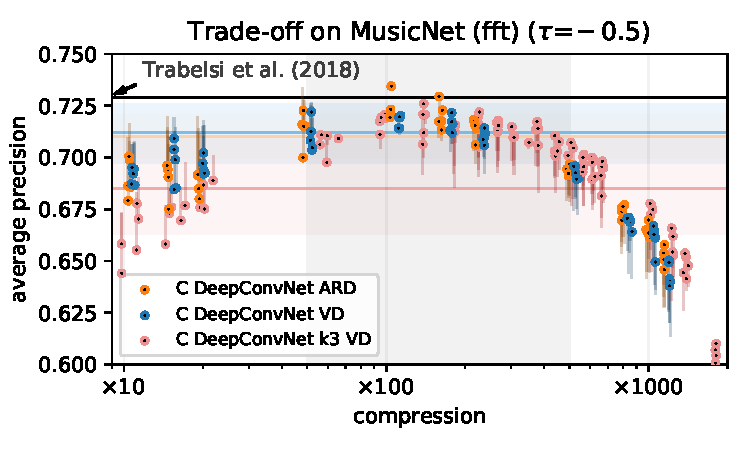
\includegraphics[scale=0.55]{figure__musicnet__trade-off/paper__musicnetram__fft__-0.5.pdf}
  \end{figure}

\end{frame}

\begin{frame}[c]{\insertsection}
  Effects of threshold selection
\end{frame}

% section results_on_musicnet (end)

\section{General Results} % (fold)
\label{sec:general_results}

\begin{frame}[c]{\insertsection}
Experiments on image classification and music transcription
\begin{itemize}
  \item $\cplx$-VD and $\cplx$-ARD equally successfully compress $\cplx$-networks
  \smallskip
  \item Variational Dropout controllably removes redundancy in wide $\cplx$ and $\real$ networks
  \smallskip
  \item $\real$-networks tend to compress better than $\cplx$-nets
\end{itemize}

\bigskip
Compression results are replicable and stable across randomizations
\begin{itemize}
  \item Fine-tuning sparse parameters generally improves performance
\end{itemize}
\end{frame}

% section general_results (end)

\section{Conclusions and Further Developments} % (fold)
\label{sec:conclusions_and_further_developments}

\begin{frame}[c]{\insertsection}
  \begin{columns}[T]
    \begin{column}{0.38\textwidth}
      \begin{itemize}
        \item Extended Bayesian Sparsification method to $\cplx$-valued networks
        \item Empirically explored the compression-performance frontier
      \end{itemize}
    \end{column}
    \begin{column}{0.58\textwidth}
      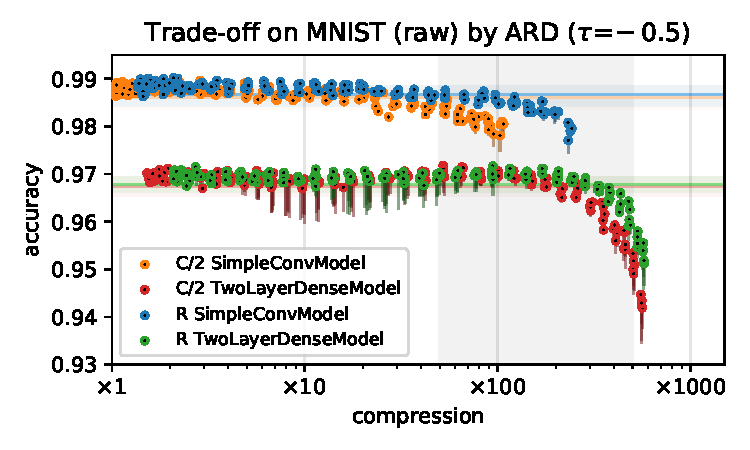
\includegraphics[scale=0.35,clip]{figure__mnist-like__trade-off/appendix__cmp__ARD__mnist__raw__-0.5.pdf}
    \end{column}
  \end{columns}

  \bigskip
  Key limitation: parameter independence % in ${\color{orange} q}$ does not hold in practice
  \begin{itemize}
    \item utilizing parameter coupling may give higher compression
    \item structured sparsity is desirable for SIMD-processing in embedded ML
  \end{itemize}

\end{frame}

% section conclusions_and_further_developments (end)

\section{References} % (fold)
\label{sec:references}

\begin{frame}[t,noframenumbering,plain,allowframebreaks]{\insertsection}
  \tiny
  \bibliographystyle{abbrvnat}
  \bibliography{presentation}
\end{frame}

% section references (end)

\end{document}
